%Este trabalho está licenciado sob a Licença Atribuição-CompartilhaIgual 4.0 Internacional Creative Commons. Para visualizar uma cópia desta licença, visite http://creativecommons.org/licenses/by-sa/4.0/deed.pt_BR ou mande uma carta para Creative Commons, PO Box 1866, Mountain View, CA 94042, USA.

\chapter{Bases e coordenadas}\label{cap_base}
\thispagestyle{fancy}

\section{Dependência linear}\label{cap_base_sec_deplinear}

\subsection{Combinação linear}

Dados vetores $\vec{u}_1$, $\vec{u}_2$, $\dotsc$, $\vec{u}_n$ e números reais $c_1$, $c_2$, $\dotsc$, $c_n$, com $n$ inteiro positivo, chamamos de
\begin{equation}
  \vec{u} = c_1\vec{u}_1 + c_2\vec{u}_2 + \cdots + c_n\vec{u}_n
\end{equation}
uma {\bf combinação linear}\index{combinação linear} de $\vec{u}_1$, $\vec{u}_2$, $\dotsc$, $\vec{u}_n$. Neste caso, também dizemos que $\vec{u}$ é {\bf gerado} pelos vetores $\vec{u}_1$, $\vec{u}_2$, $\dotsc$, $\vec{u}_n$ ou, equivalentemente, que estes vetores {\bf geram} o vetor $\vec{u}$.

\begin{ex}\label{ex:comblinear}
  Sejam dados os vetores $\vec{v}$, $\vec{w}$ e $\vec{z}$. Então, temos:
  \begin{itemize}
  \item $\vec{u}_1 = \frac{1}{2}\vec{u} + \sqrt{2}\vec{z}$ é uma combinação linear dos vetores $\vec{v}$ e $\vec{z}$.
  \item $\vec{u_2} = \vec{u} - 2\vec{z}$ é uma outra combinação linear dos vetores $\vec{v}$ e $\vec{z}$.
  \item $\vec{u_3} = 2\vec{u} - \vec{w} + \pi\vec{z}$ é uma combinação linear dos vetores $\vec{u}$, $\vec{w}$ e $\vec{z}$.
  \item $\vec{u_4} = \frac{3}{2}\vec{z}$ é uma combinação linear do vetor $\vec{z}$.
  \end{itemize}
\end{ex}

\subsection{Dependência linear}\label{cap_base_subsec_deplin}

Dois ou mais vetores dados são {\bf linearmente dependentes}\index{linearmente!dependente} (abreviação, l.d.) quando um deles for combinação linear dos demais.

\begin{ex}\label{ex:deplinear}
  No exemplo anterior (Exemplo \ref{ex:comlinear}), temos:
  \begin{itemize}
  \item $\vec{u_1}$ e $\vec{u_2}$ dependem linearmente dos vetores $\vec{u}$ e $\vec{z}$.
  \item $\vec{u_3}$ depende linearmente dos vetores $\vec{u}$, $\vec{v}$ e $\vec{z}$.
  \item Os vetores $\vec{u_4}$ e $\vec{z}$ são linearmente dependentes.
  \end{itemize}
\end{ex}

Dois ou mais vetores dados são {\bf linearmente independentes}\index{linearmente!independentes} (abreviação, l.i.)quando eles não são linearmente dependentes.

\subsection{Observações}\label{cap_base_sec_deplin_subsec_obs}

\subsubsection{Dois vetores}

Dois vetores quaisquer $\vec{u}\neq\vec{0}$ e $\vec{v}\neq\vec{0}$ são l.d. se, e somente se, qualquer uma das seguinte condições é satisfeita:
\begin{itemize}
\item um deles é combinação linear do outro, i.e.
  \begin{equation}
    \vec{u} = \alpha\vec{v}\quad\text{ou}\quad\vec{v}=\beta\vec{u};
  \end{equation}
\item $\vec{u}$ e $\vec{v}$ têm a mesma direção;
\item $\vec{u}$ e $\vec{v}$ são paralelos.
\end{itemize}

\begin{obs}
  O vetor nulo $\vec{0}$ é l.d. a qualquer vetor $\vec{u}$. De fato, temos
  \begin{equation}
    \vec{0} = 0\cdot\vec{u},
  \end{equation}
  i.e. o vetor nulo é combinação linear do vetor $\vec{u}$.
\end{obs}

\begin{obs}
  Dois vetores não nulos $\vec{u}$ e $\vec{v}$ são l.i. se, e somente se,
  \begin{equation}
    \alpha\vec{u} + \beta\vec{v} = 0 \Rightarrow \alpha=\beta=0.
  \end{equation}
  De fato, se $\alpha\neq 0$, então podemos escrever
  \begin{equation}
    \vec{u} = -\frac{\beta}{\alpha}\vec{v},
  \end{equation}
  i.e. o vetor $\vec{u}$ é combinação linear do vetor $\vec{v}$ e, portanto, estes vetores são l.d.. Isto contradiz a hipótese de eles serem l.i.. Analogamente, se $\beta \neq 0$, então podemos escrever
  \begin{equation}
    \vec{v} = -\frac{\alpha}{\beta}\vec{u}
  \end{equation}
  e, então, teríamos $\vec{u}$ e $\vec{v}$ l.d..
\end{obs}


\subsubsection{Três vetores}

Três vetores quaisquer $\vec{u}$, $\vec{v}$ e $\vec{w}$ são l.d. quando um deles pode ser escrito como combinação linear dois outros dois. Sem perda de generalidade, isto significa que existem constantes $\alpha$ e $\beta$ tais que
\begin{equation}
  \vec{u} = \alpha\vec{v} + \beta\vec{w}.
\end{equation}

Afirmamos que se $\vec{u}$, $\vec{v}$ e $\vec{w}$ são l.d., então $\vec{u}$, $\vec{v}$ e $\vec{w}$ são coplanares. Do fato de que dois vetores quaisquer são sempre coplanares, temos que $\vec{u}$, $\vec{v}$ e $\vec{w}$ são coplanares caso qualquer um deles seja o vetor nulo. Suponhamos, agora, que $\vec{u}$, $\vec{v}$ e $\vec{w}$ são não nulos e seja $\pi$ o plano determinado pelos vetores $\vec{v}$ e $\vec{w}$. Se $\alpha = 0$, então $\vec{u} = \beta\vec{w}$ e teríamos uma representação de $\vec{u}$ no plano $\pi$. Analogamente, se $\beta=0$, então $\vec{u} = \alpha\vec{v}$ e teríamos uma representação de $\vec{u}$ no plano $\pi$. Por fim, observemos que se $\alpha,\beta\neq 0$, então $\alpha\vec{v}$ tem a mesma direção de $\vec{v}$ e $\beta\vec{w}$ tem a mesma direção de $\vec{w}$. Isto é, $\alpha\vec{v}$ e $\beta\vec{w}$ admitem representações no plano $\pi$. Sejam $\overrightarrow{AB}$ e $\overrightarrow{BC}$ representações dos vetores $\alpha\vec{v}$ e $\beta\vec{w}$, respectivamente. Os pontos $A$, $B$ e $C$ pertencem a $\pi$, assim como o segmento $AC$. Como $\overrightarrow{AC} = \vec{u} = \alpha\vec{v} + \beta\vec{w}$, concluímos que $\vec{u}$, $\vec{v}$ e $\vec{w}$ são coplanares.

Reciprocamente, se $\vec{u}$, $\vec{v}$ e $\vec{w}$ são coplanares, então $\vec{u}$, $\vec{v}$ e $\vec{w}$ são l.d.. De fato, se um deles for nulo, por exemplo, $\vec{u}=\vec{0}$, então $\vec{u}$ pode ser escrito como a seguinte combinação linear dos vetores $\vec{v}$ e $\vec{w}$
\begin{equation}
  \vec{u} = 0\vec{v} + 0\vec{w}.
\end{equation}
Neste caso, $\vec{u}$, $\vec{v}$ e $\vec{w}$ são l.d.. Também, se dois dos vetores forem paralelos, por exemplo, $\vec{u}\parallel\vec{v}$, então temos a combinação linear
\begin{equation}
  \vec{u} = \alpha\vec{v} + 0\vec{w}.
\end{equation}
E, então, $\vec{u}$, $\vec{v}$ e $\vec{w}$ são l.d.. Agora, suponhamos que $\vec{u}$, $\vec{v}$ e $\vec{w}$ são não nulos e dois a dois concorrentes. Sejam, então $\overrightarrow{PA}=\vec{u}$, $\overrightarrow{PB}=\vec{v}$ e $\overrightarrow{PC}=\vec{w}$ representações sobre um plano $\pi$. Sejam $r$ e $s$ as retas determinadas por $PA$ e $PC$, respectivamente. Seja, então, $D$ o ponto de interseção da reta $s$ com a reta paralela a $r$ que passa pelo ponto $B$. Seja, também, $E$ o ponto de interseção da reta $r$ com a reta paralela a $s$ que passa pelo ponto $B$. Sejam, então, $\alpha$ e $\beta$ tais que $\alpha\vec{u}=\overrightarrow{PE}$ e $\beta\vec{w}=\overrightarrow{PD}$. Como $\vec{v} = \overrightarrow{PB} = \overrightarrow{PE} + \overrightarrow{PD} = \alpha\vec{u}+\beta\vec{w}$, temos que $\vec{v}$ é combinação linear de $\vec{u}$ e $\vec{w}$, i.e. $\vec{u}$, $\vec{v}$ e $\vec{w}$ são l.d..

\begin{obs}\label{obs:cbsc_li}
  Três vetores dados $\vec{u}$, $\vec{v}$ e $\vec{w}$ são l.i. se, e somente se, 
  \begin{equation}
    \alpha\vec{u} + \beta\vec{v} + \gamma\vec{w} = 0 \Rightarrow \alpha=\beta=\gamma = 0.
  \end{equation}
  De fator, sem perda de generalidade, se $\alpha\neq 0$, podemos escrever
  \begin{equation}
    \vec{u} = -\frac{\beta}{\alpha}\vec{v} - \frac{\gamma}{\alpha}\vec{w},
  \end{equation}
  e teríamos $\vec{u}$, $\vec{v}$ e $\vec{w}$ vetores l.d..
\end{obs}

\subsubsection{Quatro ou mais vetores}

{\bf Quatro ou mais vetores são sempre l.d..} De fato, sejam dados quatro vetores $\vec{a}$, $\vec{b}$, $\vec{c}$ e $\vec{d}$. Se dois ou três destes forem l.d. entre si, então, por definição, os quatro são l.d.. Assim sendo, suponhamos que três dos vetores sejam l.i. e provaremos que, então, o outro vetor é combinação linear desses três.

Sem perda de generalidade, suponhamos que $\vec{a}$, $\vec{b}$ e $\vec{c}$ são l.i.. Logo, eles não são coplanares. Seja, ainda, $\pi$ o plano determinado pelos vetores $\vec{a}$, $\vec{b}$ e as representações $\vec{a}=\overrightarrow{PA}$, $\vec{b}=\overrightarrow{PB}$, $\vec{c}=\overrightarrow{PC}$ e $\vec{d}=\overrightarrow{PD}$.

\begin{figure}[H]
  \centering
  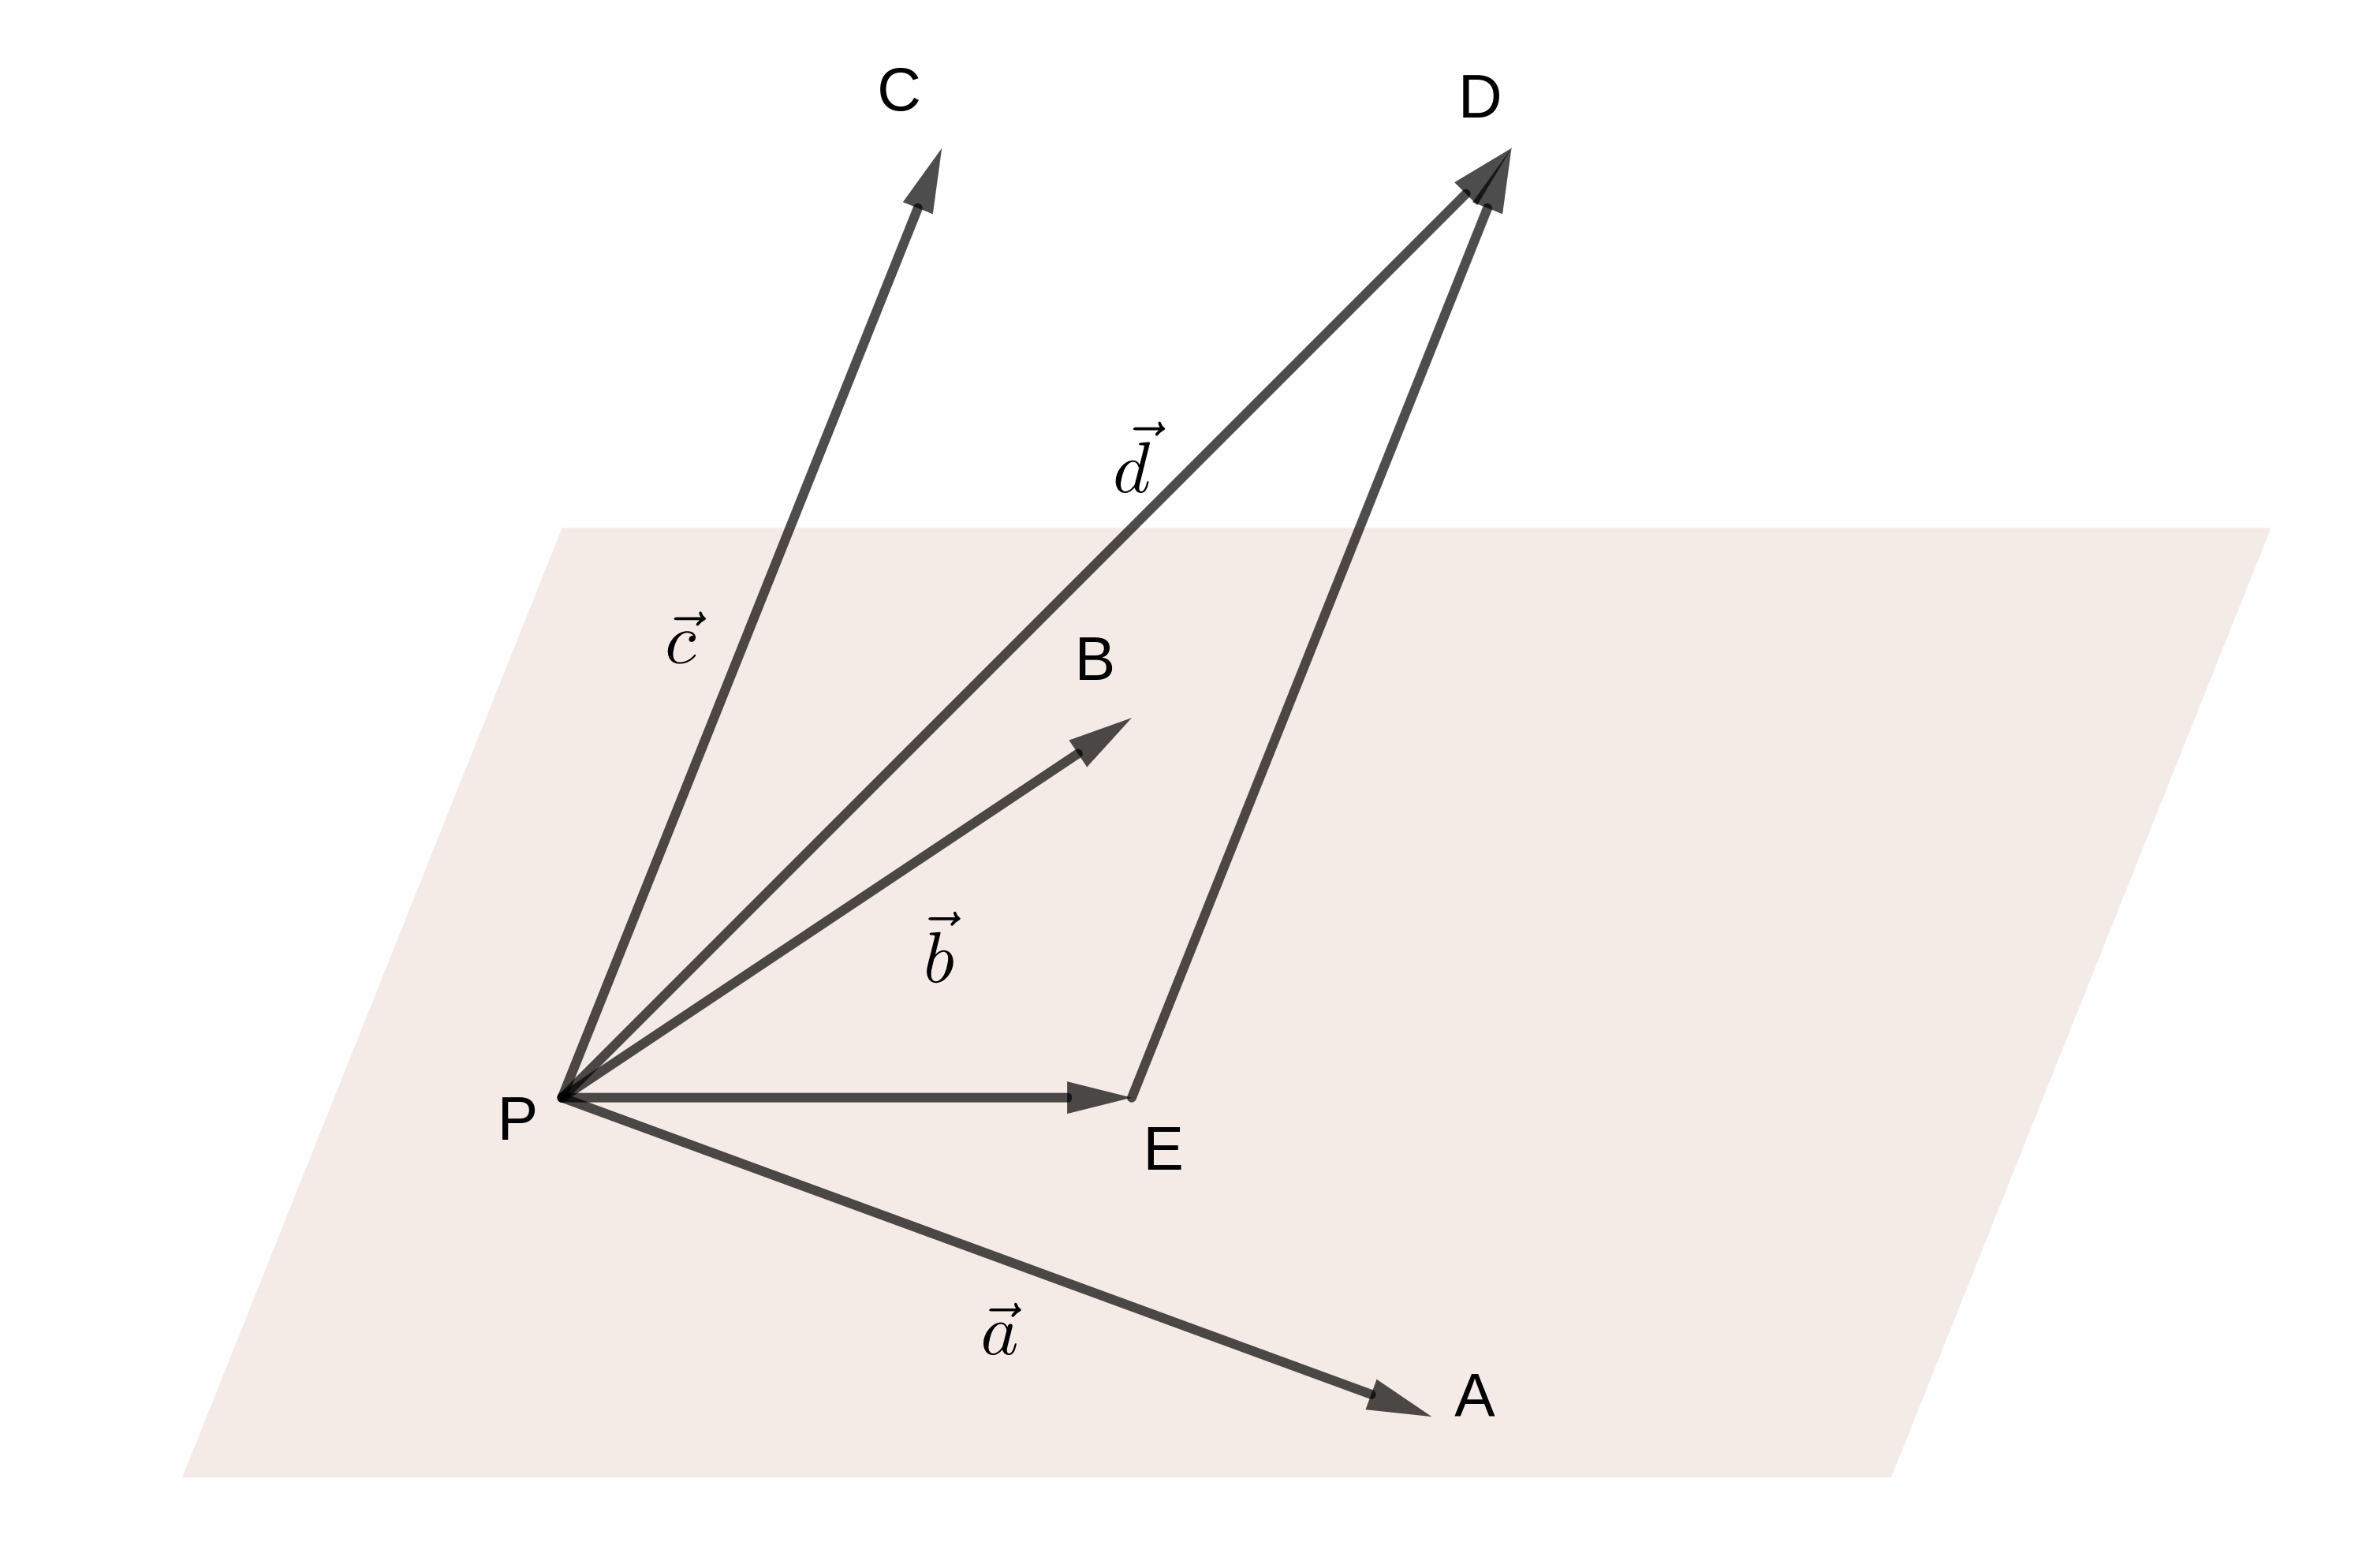
\includegraphics[width=0.7\textwidth]{./cap_base/dados/fig_4vec_ld/fig_4vec_ld}
  \caption{Quatro vetores são l.d..}
  \label{fig:4vec_ld}
\end{figure}

Consideremos a reta $r$ paralela a $\overrightarrow{PC}$ que passa pelo ponto $D$. Então, seja $E$ o ponto de interseção de $r$ com o plano $\pi$. Vejamos a Figura \ref{fig:}. Observamos que o vetor $\overrightarrow{PE}$ é coplanar aos vetores $\overrightarrow{PA}$ e $\overrightarrow{PB}$ e, portanto, exitem números reais $alpha$ e $\beta$ tal que
\begin{equation}
  \overrightarrow{PE} = \alpha\overrightarrow{PA} + \beta\overrightarrow{PB}.
\end{equation}
Além disso, como $\overrightarrow{ED}$ tem a mesma direção e sentido de $\overrightarrow{PC} = \vec{c}$, temos que
\begin{equation}
  \overrightarrow{ED} = \gamma\overrightarrow{PC}
\end{equation}
para algum número real $\gamma$. Por fim, observamos que
\begin{align*}
  \overrightarrow{PD} &= \overrightarrow{PE} + \overrightarrow{ED}\\
                      &= \alpha\overrightarrow{PA} + \beta\overrightarrow{PB} + \gamma\overrightarrow{PC}\\
                      &= \alpha\vec{a} + \beta\vec{b} + \gamma\vec{c}.
\end{align*}

\subsection*{Exercícios}

\begin{exer}
  Sendo $\overrightarrow{AB} + 2\overrightarrow{BC} = \vec{0}$, mostre que $\overrightarrow{PA}$, $\overrightarrow{PB}$ e $\overrightarrow{PC}$ são l.d. para quaquer ponto $P$.
\end{exer}
\begin{resp}
  Dica: os vetores $\overrightarrow{AB}$ e $\overrightarrow{BC}$ são l.d..
\end{resp}

\begin{exer}
  Sejam dados três vetores quaisquer $\vec{a}$, $\vec{b}$ e $\vec{c}$. Mostre que os vetores $\vec{u} = 2\vec{a}-\vec{b}$, $\vec{v}=-\vec{a}-2\vec{c}$ e $\vec{w}=\vec{b}+4\vec{c}$ são l.d..
\end{exer}
\begin{resp}
  Dica: Escreva um dos vetores como combinação linear dos outros.
\end{resp}

\emconstrucao

\section{Bases e coordenadas}\label{cap_base_sec_base}

Seja $V$ o conjunto de todos os vetores no espaço tridimensional. Conforme discutido na Subseção \ref{cap_base_subsec_deplin}, se $\vec{a}$, $\vec{b}$ e $\vec{c}$ são l.i., então qualquer vetor $\vec{u}\in V$ pode ser escrito como uma combinação linear destes vetores, i.e. existem números reais $\alpha$, $\beta$ e $\gamma$ tal que
\begin{equation}
  \vec{u} = \alpha\vec{a} + \beta\vec{b} + \gamma\vec{c}.
\end{equation}

A observação acima motiva a seguinte definição: uma {\bf base}\index{base} de $V$ é uma sequência de três vetores l.i. de $V$.

Seja $B = (\vec{a}, \vec{b}, \vec{c})$ uma dada base de $V$. Então, dado qualquer $\vec{v}\in V$, existe um único terno de números reais $\alpha$, $\beta$ e $\gamma$ tais que
\begin{equation}
  \vec{v} = \alpha\vec{a} + \beta\vec{b} + \gamma\vec{c}.\label{clsb_eq0}
\end{equation}
De fato, a existência de $alpha$, $\beta$ e $\gamma$ segue imediatamente do fato de que $\vec{a}$, $\vec{b}$ e $\vec{c}$ são l.i. e, portanto, $\vec{v}$ pode ser escrito como uma combinação linear destes vetores. Agora, para verificar a unicidade de $alpha$, $\beta$ e $\gamma$, tomamos $\alpha'$, $\beta'$ e $\gamma'$ tais que
\begin{equation}
  \vec{v} = \alpha'\vec{a} + \beta'\vec{b} + \gamma'\vec{c}.\label{clsb_eq1}
\end{equation}
Subtraindo \eqref{clsb_eq1} de \eqref{clsb_eq0}, obtemos
\begin{equation}
  \vec{0} = (\alpha-\alpha')\vec{a}+(\beta-\beta')\vec{b}+(\gamma-\gamma')\vec{c}.
\end{equation}
Como $\vec{a}$, $\vec{b}$ e $\vec{c}$ são l.i., segue que\footnote{Lembre-se da Observação \ref{obs:cbsc_li}.}
\begin{equation}
  \alpha-\alpha'=0,~\beta-\beta'=0,~\gamma-\gamma'=0,
\end{equation}
i.e. $\alpha=\alpha'$, $\beta=\beta'$ e $\gamma=\gamma'$.

\begin{figure}[H]
  \centering
  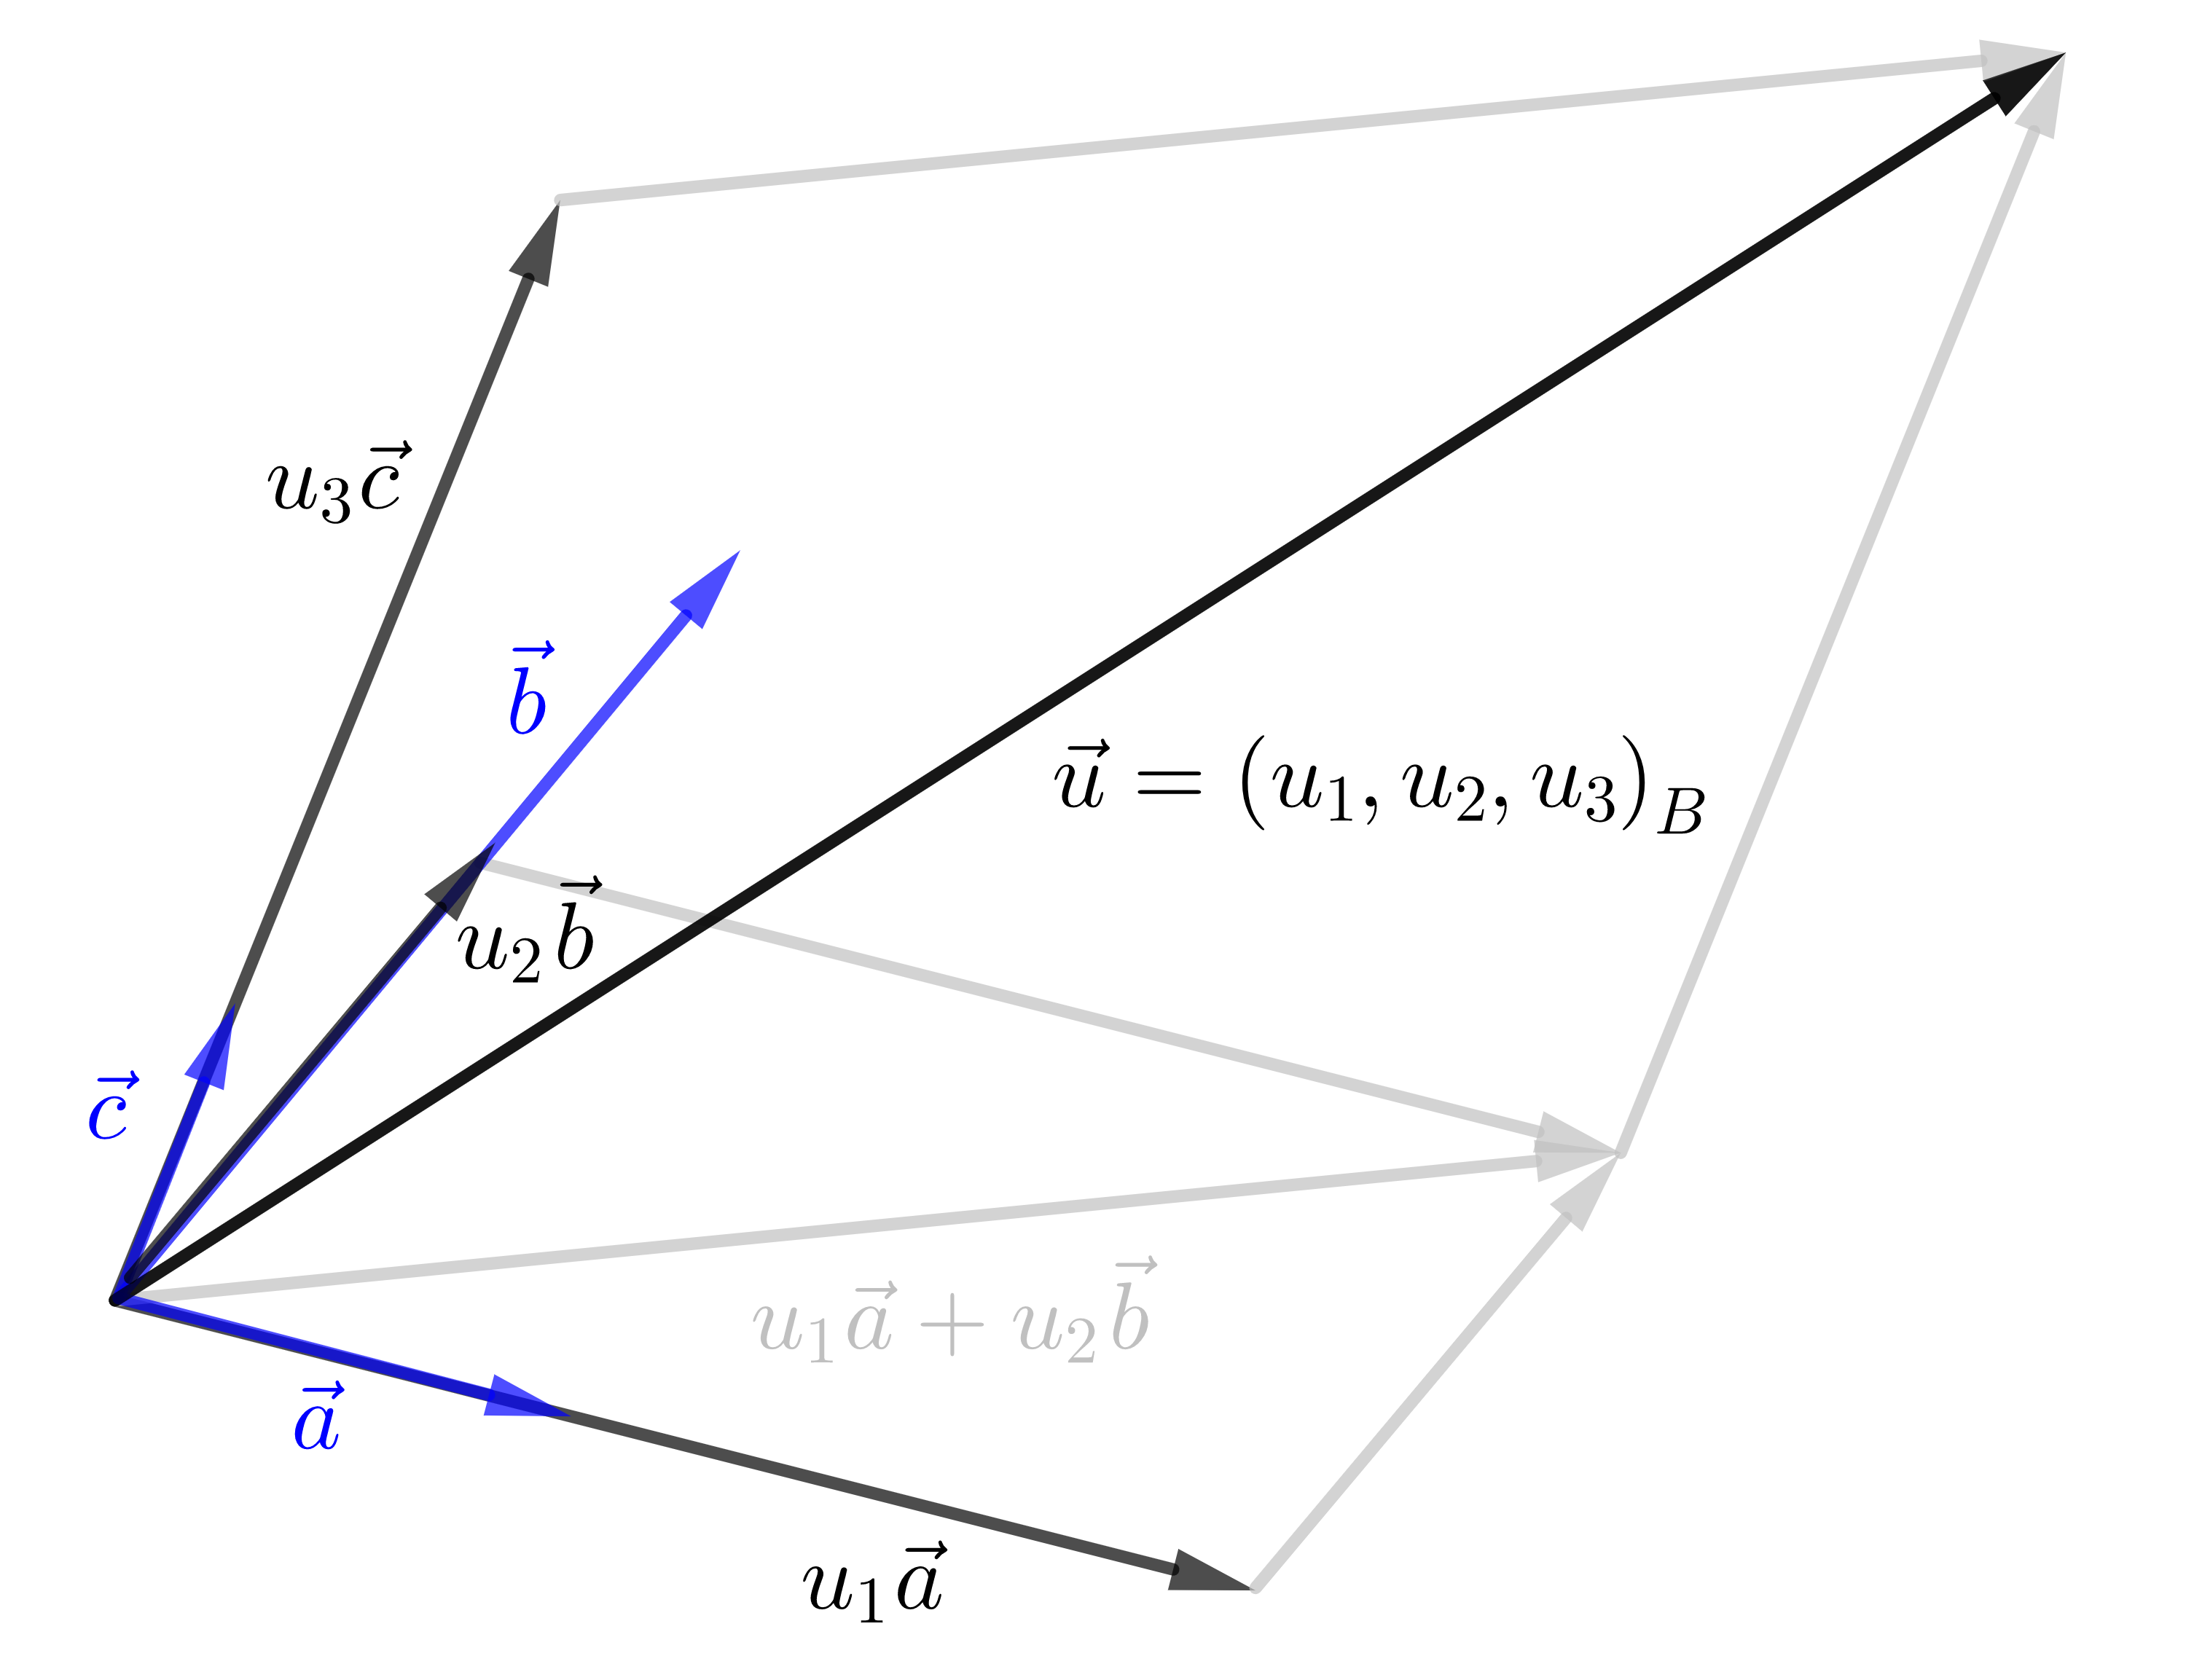
\includegraphics[width=0.7\textwidth]{./cap_base/dados/fig_coord/fig_coord}
  \caption{Representação de um vetor $\vec{u} = (u_1, u_2, u_3)_B$ em uma dada base $B=(\vec{a},\vec{b},\vec{c})$.}
  \label{fig:coord}
\end{figure}

Com isso, fixada uma base $B = (\vec{a}, \vec{b}, \vec{c})$, cada vetor $\vec{u}$ é representado de forma única como combinação linear dos vetores da base, digamos
\begin{equation}
  \vec{u} = u_1\vec{a} + u_2\vec{b} + u_3\vec{c},
\end{equation}
onde $u_1$, $u_2$ e $u_3$ são números reais fixos, chamados de {\bf coordenadas}\index{coordenadas} do $\vec{u}$ na base $B$. Ainda, usamos a notação
\begin{equation}
  \vec{u} = (u_1, u_2, u_3)_B,
\end{equation}
para expressar o vetor $\vec{u}$ nas suas coordenadas na base $B$. Vejamos a Figura \ref{fig:coord}.

\begin{ex}
  Fixada uma base $B = (\vec{a}, \vec{b}, \vec{c})$, o vetor $\vec{u}$ de coordenadas $\vec{u}=(-2,\sqrt{2},-3)$ é o vetor $\vec{u} = -2\vec{a} + \sqrt{2}\vec{b} - 3\vec{c}$.
\end{ex}

\subsection{Operações de vetores com coordenadas}


Na Seção \ref{cap_vetor_sec_vetor}, definimos as operações de adição, subtração e multiplicação por escalar do ponto de vista geométrico. Aqui, veremos como estas operação são definidas a partir das coordenadas de vetores.

Sejam $B = (\vec{a}, \vec{b}, \vec{c})$ uma base de $V$ e os vetores $\vec{u} = (u_1, u_2, u_3)_B$ e $\vec{v} = (v_1, v_2, v_3)_B$. Isto é, temos
\begin{align}
  \vec{u} &= u_1\vec{a} + u_2\vec{b} + u_3\vec{c},\\
  \vec{v} &= v_1\vec{a} + v_2\vec{b} + v_3\vec{c}.
\end{align}
Então, a {\bf adição} de $\vec{u}$ com $\vec{v}$ é a soma
\begin{align}
  \vec{u}+\vec{v} &= \underbrace{u_1\vec{a} + u_2\vec{b} + u_3\vec{c}}_{\vec{u}} + \underbrace{v_1\vec{a} + v_2\vec{b} + v_3\vec{c}}_{\vec{v}}\\
  &= (u_1+v_1)\vec{a} + (u_2+v_2)\vec{b} + (u_3+v_3)\vec{c},
\end{align}
ou seja
\begin{equation}
  \vec{u}+\vec{v}=(u_1+v_1, u_2+v_2, u_3+v_3)_B.
\end{equation}

\begin{ex}
  Fixada uma base qualquer $B$ e dados os vetores $\vec{u} = (2, -1, -3)_B$ e $\vec{v} = (-1, 4, -5)_B$, temos
  \begin{equation}
    \vec{u}+\vec{v} = \left(2+(-1), -1+4, -3+(-5)\right)_B = (1,3,-8)_B.
  \end{equation}
\end{ex}

De forma, análoga, o {\bf vetor oposto} ao vetor $\vec{u}$ é
\begin{align}
  -\vec{u} &= -(\underbrace{u_1\vec{a} + u_2\vec{b} + u_3\vec{c}}_{\vec{u}})\\
           &= (-u_1)\vec{a} + (-u_2)\vec{b} + (-u_3)\vec{c},
\end{align}
ou seja,
\begin{equation}
  -\vec{u} = (-u_1, -u_2, -u_3)_B.
\end{equation}

\begin{ex}
  Fixada uma base qualquer $B$ e dado o vetor $\vec{v} = (2, -1, -3)_B$, temos
  \begin{equation}
    -\vec{v} = \left(-2, 1, 3\right)_B.
  \end{equation}
\end{ex}


Lembrando que {\bf subtração} de $\vec{u}$ com $\vec{v}$ é $\vec{u}-\vec{v} := \vec{u} + (-\vec{v})$, segue
\begin{equation}
  \vec{u}-\vec{v} = (u_1-v_1, u_2-v_2, u_3-v_3)_B.
\end{equation}

\begin{ex}
  Fixada uma base qualquer $B$ e dados os vetores $\vec{u} = (2, -1, -3)_B$ e $\vec{v} = (-1, 4, -5)_B$, temos
  \begin{equation}
    \vec{u}-\vec{v} = \left(2-(-1), -1-4, -3-(-5)\right)_B = (3,-5,2)_B.
  \end{equation}
\end{ex}


Com o mesmo raciocínio, fazemos a {\bf multiplicação de} um dado {\bf número} $\alpha$ pelo {\bf vetor} $\vec{u}$. Vejamos, por definição,
\begin{align}
  \alpha\vec{u} &= \alpha(\underbrace{u_1\vec{a} + u_2\vec{b} + u_3\vec{c}}_{\vec{u}})\\
                &= (\alpha u_1)\vec{a} + (\alpha u_2)\vec{b} + (\alpha u_3)\vec{c},
\end{align}
ou seja,
\begin{equation}
  \alpha\vec{u} = (\alpha u_1,\alpha u_2, \alpha u_3).
\end{equation}

\begin{ex}
  Fixada uma base qualquer $B$ e dado o vetor $\vec{v} = (2, -1, -3)_B$, temos
  \begin{equation}
    \frac{1}{3}\vec{v} = \left(-\frac{2}{3}, \frac{1}{3}, 1\right)_B.
  \end{equation}
\end{ex}

\subsection{Dependência linear}

\subsubsection{Dois vetores}

Na Subseção \ref{cap_base_sec_deplin_subsec_obs}, discutimos que dois vetores $\vec{u}$, $\vec{v}$ são l.d. se, e somente se, um for múltiplo do outro, i.e. existe um número real $\alpha$ tal que
\begin{equation}\label{eq:cbsb_vmv}
  \vec{u} = \alpha\vec{v},
\end{equation}
sem perda de generalidade\footnote{Formalmente, pode ocorrer $\vec{v} = \beta\vec{u}$.}.

Fixada uma base $B = (\vec{a}, \vec{b}, \vec{c})$, temos $\vec{u} = (u_1, u_2, u_3)_B$ e $\vec{v} = (v_1, v_2, v_3)_B$. Com isso, a equação \eqref{eq:cbsb_vmv} pode ser reescrita como
\begin{equation}
  (u_1, u_2, u_3)_B = \alpha(v_1, v_2, v_3)_B = (\alpha v_1, \alpha v_2, \alpha v_3)_B,
\end{equation}
donde
\begin{equation}
  u_1 = \alpha v_1,~u_2 = \alpha v_2,~u_3 = \alpha v_3.
\end{equation}
Ou seja, dois vetores são linearmente dependentes se, e somente se, as coordenadas de um deles forem, respectivamente, múltiplas (de mesmo fator) das coordenadas do outro.

\begin{ex}
  Vejamos os seguintes casos:
  \begin{enumerate}[a)]
  \item $\vec{u} = (2,-1,-3)$ e $\vec{v} = \left(1,-\frac{1}{2},-\frac{3}{2}\right)$ são l.d., pois
    \begin{equation}
      2 = 2\cdot \frac{1}{2},~-1 = 2\cdot\left(-\frac{1}{2}\right),~-3 = 2\cdot\left(-\frac{3}{2}\right).
    \end{equation}
  \item $\vec{u} = (2,-1,-3)$ e $\vec{v} = \left(2,-\frac{1}{2},-\frac{3}{2}\right)$ são l.i., pois $u_1 = 1\cdot v_1$, enquanto $u_2 = 2v_2$.
  \end{enumerate}
\end{ex}

\subsubsection{Três vetores}

Na Subseção \ref{cap_base_sec_deplin_subsec_obs}, discutimos que três vetores $\vec{u}$, $\vec{v}$ e $\vec{w}$ são l.i. se, e somente se,
\begin{equation}
  \alpha\vec{u}+\beta\vec{v}+\gamma\vec{w}=\vec{0} \Rightarrow \alpha=\beta=\gamma.
\end{equation}

Seja, então, $B = (\vec{a}, \vec{b}, \vec{c})$ uma base de $V$. Então, temos que a equação
\begin{equation}
  \alpha\vec{u}+\beta\vec{v}+\gamma\vec{w} = \vec{0}
\end{equation}
é equivalente a
\begin{equation}
  \alpha(u_1,u_2,u_3)+\beta(v_1,v_2,v_3)+\gamma(w_1,w_2,w_3)=(0, 0, 0).
\end{equation}
Esta por sua vez, nos leva ao seguinte sistema linear
\begin{equation}
  \left\{
    \begin{array}{l}
      u_1\alpha + v_1\beta + w_1\gamma = 0\\
      u_2\alpha + v_2\beta + w_2\gamma = 0\\
      u_3\alpha + v_3\beta + w_3\gamma = 0
    \end{array}
  \right.
\end{equation}
Lembremos que um tal sistema tem solução única (trivial) se, e somente se, o determinante de sua matriz dos coeficientes é nulo, i.e.
\begin{equation}
  \left|\begin{array}{ccc}
    u_1 & v_1 & w_1\\
    u_2 & v_2 & w_2\\
    u_3 & v_3 & w_3
  \end{array}\right| \neq 0.
\end{equation}

\begin{ex}
  Fixada uma base $B$ de $V$, sejam os vetores $\vec{u} = (2,1,-3)$, $\vec{v} = (1,-1,2)$ e $\vec{w} = (-2,1,1)$. Como
  \begin{align}
    \left|\begin{array}{ccc}
            u_1 & v_1 & w_1\\
            u_2 & v_2 & w_2\\
            u_3 & v_3 & w_3
          \end{array}\right| &=
                               \left|\begin{array}{ccc}
                                       2 & 1 & -2\\
                                       1 & -1 & 1\\
                                       -3 & 2 & 1
                                     \end{array}\right| \\
    &= -2-4-3+6-4-1 = -8\neq 0.
  \end{align}
\end{ex}

\subsection*{Exercícios}

\emconstrucao

\section{Mudança de base}

\emconstrucao